\section{\Large CONTROL}
\subsection{Actuator Specifications}
We size reaction wheels, magnetorquers, and thrusters in this section. For this problem set, we only simulate the reaction wheels, but we may include magnetorquers and thrusters later.

The calculations for actuator sizing are based on the worst case disturbance torque ($M_d$), orbit period ($P$), largest expected magnetic field ($B$), and estimated moment arm of a thruster ($b$). This is used to find the required momentum storage of a reaction wheel ($L$), required dipole of a magnetorquer ($D$), and required thrust of a thruster ($T$), based on the equations below. These values are presented in Table \ref{tab:estimate_actuator_sizing}.
\begin{align*}
    L &= \frac{M_d P}{4 \sqrt{2}} \\
    D &= \frac{M_d}{B} \\
    T &= \frac{M_d}{b}
\end{align*}
\vspace{-2em}
\begin{table}[H]
\centering
\caption{Actuator Parameters for Disturbance Rejection}
\label{tab:estimate_actuator_sizing}
\begin{tabular}{|l|l|l|}
\hline
L [Nms] & D [A\/m\textsuperscript{2}] & T [N]    \\ \hline
2.5392    & 55.0737   & 0.004        \\ \hline
\end{tabular}
\end{table}

In addition to disturbance rejection, the actuators should also be sized in order to perform necessary maneuvers, meaning that the values in Table \ref{tab:estimate_actuator_sizing} may need to be greater when considering all the operational modes of the satellite ADCS system. The NISAR satellite uses four $50 N m s$ reaction wheels, a combination of three $565 A m^2$ and $350 A m^2$ magnetorquers, and four $1 N$ thrusters for attitude control \cite{NISARMission}. Using these metrics, we found equivalent commercially available actuators to estimate other key actuator parameters. For reaction wheels, we referenced the ASTROFEIN RW3000, which has properties listed in Table \ref{tab:reaction_wheel_data}. For thrusters, we referenced the Ariane Group 1N Hydrazine Thruster, which has properties listed in Table \ref{tab:reaction_thruster}. For the magnetorquer, we only require the dipole moment to perform our sizing.

\begin{table}[H]
\centering
\caption{RW 3000 Reaction Wheel Data \cite{RW3000Datasheet}}
\label{tab:reaction_wheel_data}
\begin{tabular}{|l|l|l|l|}
\hline
Model Name & Momentum     & Moment of Inertia    & Maximum RPM \\ \hline
RW 3000    & $\qty{50}{Nms}$   & $\qty{0.119}{kg m^2}$       & $4000$        \\ \hline
\end{tabular}
\end{table}

\begin{table}[H]
\centering
\caption{Ariane Group Thruster Data}
\label{tab:reaction_thruster}
\begin{tabular}{|l|l|l|}
\hline
Model Name              & Thrust (T)    & Specific Impulse (I\textsubscript{sp})\\ \hline
1N Hydrazine Thruster   & 1 N           & 220 s \\ \hline
\end{tabular}
\end{table}

\subsection{Actuator Models}
Our actuator model accepts $M_{c}$ as a torque command from the control law and tracks the angular momentum state of our reaction wheels. We can propagate the angular momentum by computing the rate of change of the angular momentum. This is also equivalent to commanding a change in angular velocity of the reaction wheels.
\begin{align*}
    \Dot{\Vec{L}}_{w} &= \Vec{A}^{*} (-\Vec{M}_{c} - \Vec{\omega} \times \Vec{A} \Vec{L}_{w})
\end{align*}
We can incorporate estimation error by passing in $\omega_{est}$ when computing $\Dot{\Vec{L}}_{w}$, and then propagating the dynamics using $\omega_{true}$ in the same formula for $\Vec{M}_{c}$.

For the layout of our system. We position four reaction wheels in a tetrahedral configuration–this system is overactuated but allows for redundancy in case of reaction wheel failure. Our mounting matrix is as follows:
\begin{equation*}
    \Vec{A} = \frac{1}{\sqrt{3}} \begin{bmatrix}
        -1 & 1 & 1 & -1 \\
        -1 & -1 & 1 & 1 \\
        1 & 1 & 1 & 1
    \end{bmatrix}
\end{equation*}
Prior to implementing the control law, we use an arbitrary sinusoidal signal as our torque command and plot the resulting angular velocities of our reaction wheels. This output is coupled with our simulation of the spacecraft dynamics.

\begin{figure}[H]
\centering
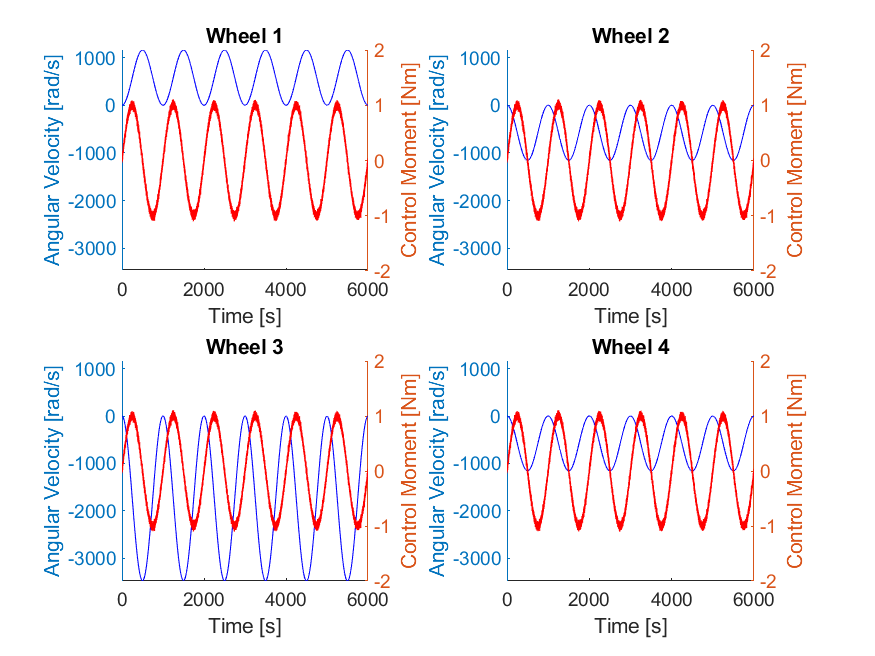
\includegraphics[scale=0.9]{Images/ps9_problem2.png}
\caption{Reaction wheel angular velocities for arbitary control moment inputs}
\label{fig:ps9_problem2}
\end{figure}

\subsection{Control Law}
We implement the control law using the following equations, where $f$ is frequency of the actuator response and $I_{i}$ is the moment of inertia about principal axis $i$. The control law differs slightly for each axis based on the moment of inertia about that axis.
\begin{align*}
    M_{c,i} &= -K_{p,i} \alpha_{i} - K_{d,i} \Dot{\alpha}_{i} \\
    K_{p,i} &= \frac{f^{2}}{I_{i}} \\
    K_{d,i} &= 2 \sqrt{I_{i} \left[ 3 n^{2} (I_{k} - I_{j}) + K_{p,i} \right]}
\end{align*}
To obtain small angle $\alpha_{i}$, we compute the rotation between the current attitude and the target attitude by using the direction cosine matrices of each relative to the inertial frame. From this new rotation $A_{E}$ from target attitude to current attitude, we can directly extract $\alpha_{x}$, $\alpha_{y}$, and $\alpha_{z}$ from the corresponding indices in the matrix to create our linear control law. Similarly, for a nonlinear control law, we can used the following formula.
\begin{align*}
    \Vec{M}_{c,i} &= -K_{p,i} \frac{A_{E,jk} - A_{E,kj}}{2} - K_{d,i} \omega_{i}
\end{align*}
This formula effectively takes an average of the relevant indices for each $\alpha_{i}$ in $A_{E}$. Before adding sensor errors, we obtain the following control result for our desired (originally unstable) Earth-pointing attitude, which we have detailed previously in this report.

\begin{figure}[H]
\centering
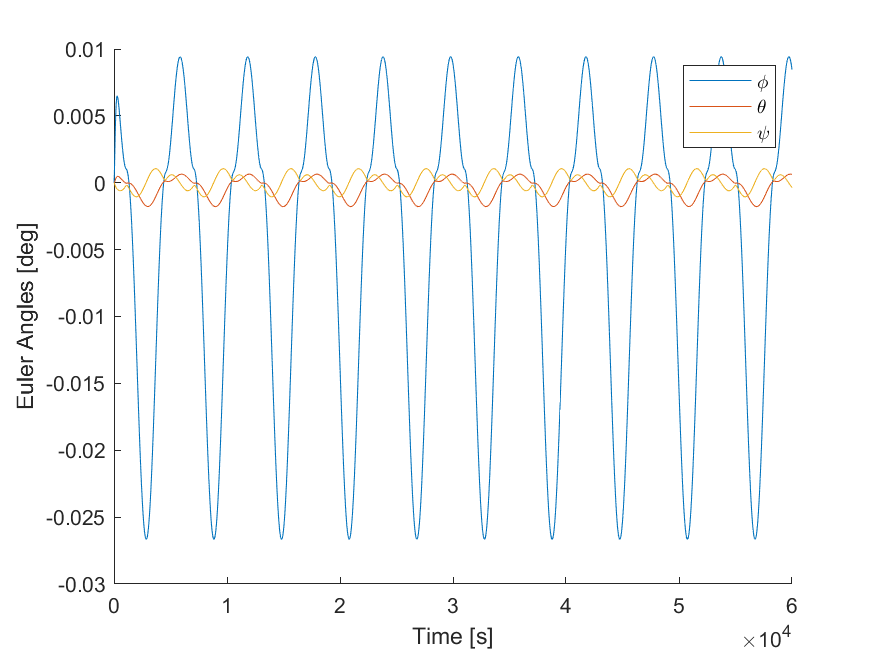
\includegraphics[scale=0.7]{Images/ps9_problem3_controlError_nonlinear_GT.png}
\caption{Control error over 10 orbits without sensor errors}
\label{fig:ps9_problem3_controlError_nonlinear_GT}
\end{figure}

\subsection{Control and Estimation Errors}
Upon adding state estimation error, our control error changes, as shown in Figure \ref{fig:ps9_problem3_controlError_nonlinear} Note that we are implementing the nonlinear control law here, but we also have implemented the linear control law and obtained nearly identical results–this is as expected, since we are attempting to reject small disturbances, and the difference between the linear and nonlinear control laws should be approximately zero in this regime.

\begin{figure}[H]
\centering
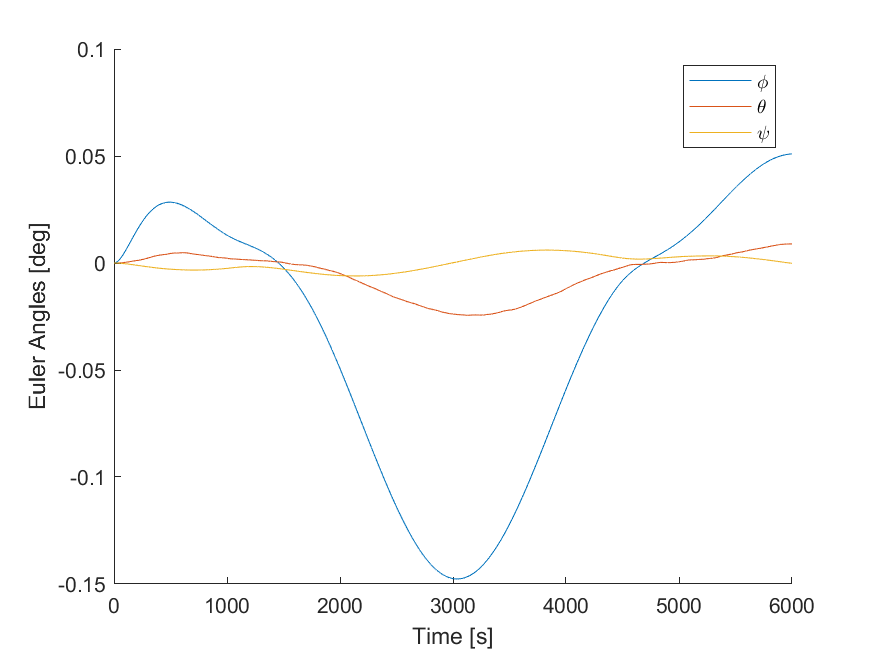
\includegraphics[scale=0.7]{Images/ps9_problem3_controlError_nonlinear.png}
\caption{Angular error relative to target attitude over 10 orbits}
\label{fig:ps9_problem3_controlError_nonlinear}
\end{figure}

\begin{figure}[H]
\centering
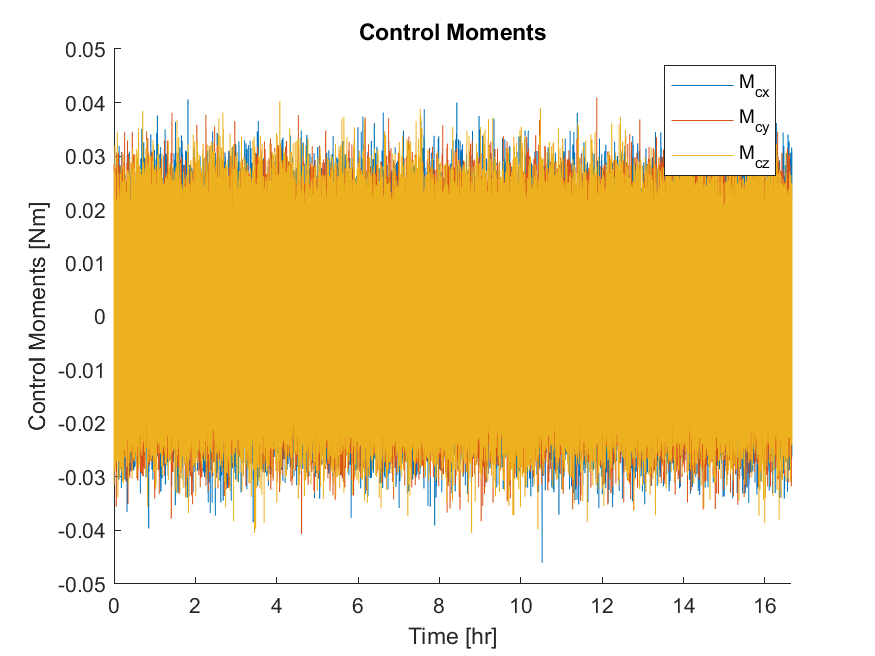
\includegraphics[scale=0.7]{Images/ps9_problem3_controlMoments_nonlinear.png}
\caption{Control torque commands over 10 orbits}
\label{fig:ps9_problem3_controlMoments_nonlinear}
\end{figure}

For simply pointing the radar instrument directly at the ground below, we are able to meet the NISAR pointing requirement of less than 273 arcsec (approximately 0.075 degrees). In Figure \ref{fig:ps9_problem3_controlMoments_nonlinear}, we show the torque commands issued by our control law. We also show the attitude determination error based on our filter in Figure \ref{fig:ps9_problem3_determinationError_nonlinear}.

\begin{figure}[H]
\centering
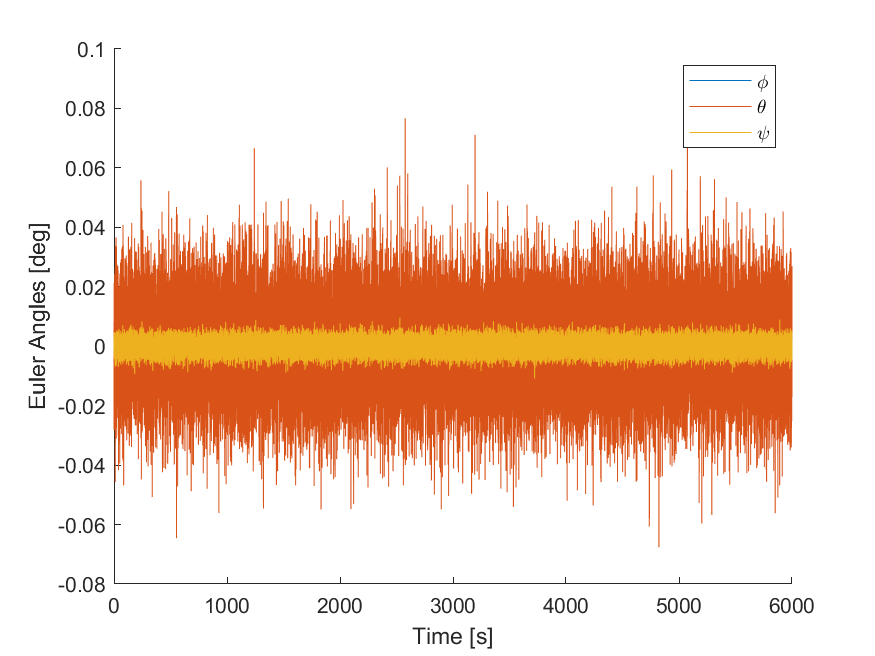
\includegraphics[scale=0.7]{Images/ps9_problem3_determinationError_nonlinear.png}
\caption{Attitude determination error over 10 orbits}
\label{fig:ps9_problem3_determinationError_nonlinear}
\end{figure}

In Figure \ref{fig:ps9_problem3_wheelMomentum_nonlinear}, we can see that the angular velocities of our four reaction wheels grow over time. This will eventually lead to saturation and require desaturation over longer periods of time.

\begin{figure}[H]
\centering
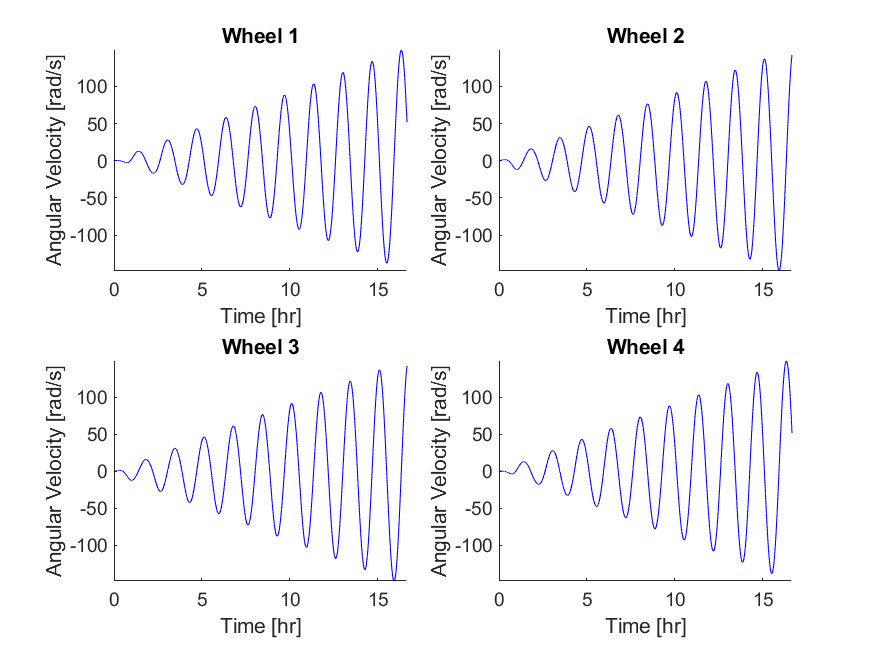
\includegraphics[scale=0.7]{Images/ps9_problem3_wheelMomentum_nonlinear.png}
\caption{Reaction wheel angular velocity over 10 orbits}
\label{fig:ps9_problem3_wheelMomentum_nonlinear}
\end{figure}